\chapter{Experiments}

In this chapter, we will introduce the experiments we conducted on aspect extraction for product reviews. We will talk about two experiments we carried out. The first one is a comparison of several methods for the vetcor representation of sentences. Since in our multistage clustering framekwork, we need to first transform the sentences into vectors, the way we represent the sentences is crucial to the performance of the whole model. In particular, we need the vector representation to accurately capture the semantic similarity between sentences, so we test the performance of the methods on a sentence similarity prediction task. The second experiments

\section{Experiment 1: A Comparison of Sentence Vectors}

The vector representation of sentences is a crucial module of our framework, so we conduct this experiment to find a proper method. There are mainly two methods we want to compare, recurrent neural network and paragraph vector. 

To use recurrent nerual network for sentence vectors, we train a language model on the corpus. After the perplexity converges, we use the trained network to process each sentence of the corpus and take the last hidden vector as the vector representation of the sentence. Using paragraph vector is easier because the vector representation is directly stored in the model's parameters. We only need to train until the log-likelihood converges and take the parameter matrix for the sentence vectors.

Since we use the sentence vectors for clustering the sentences based on their topics, and K-Means algorithm uses the distances between the vectors to determine which cluster each sentence belongs to, we need the sentence vectors to accurately capture the semantic distance between the sentences. For this purpose, we test how well the vector representations capture the semantic similarity, that is, a sentence similarity prediction task. We follow SemEval-2015 Task 2: Semantic Textual Similarity \cite{agirrea2015semeval}, which uses a dataset of 14250 (11250 for train and 3000 for test) sentence pairs for the English subtask. We train our model on all the sentences and test on the 3000 sentence pairs from the test set.

For each sentence pair, both neural network models give us the independent sentence vectors; to use this pair of vectors to predict the semantic similarity, we train a predictor backend. This backend is a three-layer feed-forward neural network, which takes a pair of sentences as input, and output a score from 0 to 5. The backend is trained independently for both RNN and paragraph vector, with the same input dimensionality and network structure, for the same number of iterations. 

In our experiments, both the RNN hidden vectors and the paragraph vectors are 300-dimensional; the hidden layer of the predictor backend is 100-dimensional. We also compare the neural network models with an SVM with gaussian kernel as a non-neural baseline. The results on SemEval-2015 English subtask dataset is shown in Table~\ref{table:semeval}

\begin{table}
\centering
\begin{tabular}{|l|c|c|}
    \hline
    Model & Train F1 & Test F1 \\ \hline\hline
    SVM & 0.235 & 0.242 \\ \hline
    RNN & 0.341 & 0.270 \\ \hline
    LSTM & 0.481 & 0.324 \\ \hline
    PV & 0.812 & 0.338 \\ \hline
    LSTM+ff & 0.596 & 0.491 \\ \hline
\end{tabular}
\caption{F1 scores on training set and test set.}
\label{table:semeval}
\end{table}

It can be seen that, all the neural network models outperformed the more traditional SVM method, demonstrating that neural networks can truly improve the performance of natural language processing tasks. We can also see that, LSTM improved significantly against vanilla RNN, with its more complicated connections and gates that help deal with the vanishing gradient problem. We can also see that, although with a much simpler design and less parameters, paragraph vectors outperformed LSTM on this task. It is possible that the last hidden vector of RNN is not a proper representation of the sentence for the semantic similarity task, probabily due to its emphasis on the last seen words than earlier words. But we also note that, we can extend the LSTM structure specifically for this task: as shown in the last row, instead of training the LSTM for a language model, we train the LSTM reader of the sentence pair and the predictor backend simultaneously; with doubled parameters, we acheived much better performance. By training the LSTM sentence reader and the predictor neural network end-to-end, the LSTM reader can be informed about which words are important to predicting the semantic similarity during the back-propagation. Note that this flexibility does not apply to paragraph vector, which is a strictly unsupervised model.

\section{Experiment 2: End-to-end Aspect Extraction}

In this experiment, we test the performance of our system on the real-life application it is designed for, the aspect extraction task for user reviews. We will first talk about the data we use in the experiment, which is gather by the author from various e-commerace websites. On most of these websites, there is either no review summarization available, or there is only a rather simplistic phrase-based summarization, which is not very informative and helpful to the consumers. We will introduce two metrics designed for measuring the accuracy extraction, hit-by-first rate and smoothed aspect score. Besides quantitatively comparing our model with others on these metrics, we also evaluate our model qualitatively: we will demonstarte that, combined with a sentiment prediction backend, our framework can provide a complete aspect-based summarization that is much more informative and clear than what is now available on most websites.

\subsection{Data}

The data we use in this experiment is gathered from various websites, including Amazon.com, TripAdvisor.com, etc. The reviews are about various types of products. Some of the reviews come with extra information such as the general ratings but we only use the review text, which is plain English. We do not use any labels for our model, the human labels are only used for evaluation purpose. The product category and number of reviews are shown in Table~\ref{table:dataset}

For evaluation, we asked 5 labelers to provide aspect words for each product type. We don't give any instruction about how many aspects should be provided for each product type (more on this later). After they provide their choices of aspects independently, we count the appearances of each aspect word. The number of appearances of each aspect is used as a score for that aspect w.r.t. the product type; for example, if 4 out of 5 labelers think ``food" should be an aspect for product type ``hotel", then aspect ``food" has score 4 for hotels (all aspect scores range from 0 to 5). We only consider aspects with score higher than 2 to be effective, because these are agreed upon by at least 2 labelers. We use the effective aspects as the ground-truth. The information about the dataset and the final number of aspects are summarized in Table~\ref{table:dataset}. Examples of labeling result (aspect words and scores) for product category hotel, mobile phone and movie are shown in Table~\ref{table:data_example}.

\begin{table}
\centering
\begin{tabular}{|l|ccccc|}
\hline
Product type     & hotel & mobile phone & mp3 player & laptop    & tv   \\
No. of reviews   & 27145 & 3716         & 2745       & 5471      & 1237 \\
Words per review & 210   & 136          & 128        & 97        & 102  \\
No. of aspects   & 7     & 8            & 8          & 9         & 8    \\\hline\hline
Product type     & movie & car          & shoes      & headphone & gps  \\
No. of reviews   & 3000  & 1074         & 1748       & 1647      & 1726 \\
Words per review & 194   & 147          & 82         & 122       & 72   \\
No. of aspects   & 8     & 9            & 8          & 6         & 6   \\ \hline
\end{tabular}
\caption{Dataset information.}
\label{table:dataset}
\end{table}

\begin{table}
\centering
\begin{tabular}{|lc|lc|lc|}
\hline
Aspect   & Score & Aspect   & Score & Aspect   & Score \\\hline
room     & 5     & screen   & 5     & actor    & 5     \\
service  & 5     & battery  & 5     & story    & 4     \\
bed      & 4     & service  & 3     & director & 4     \\
location & 4     & quality  & 3     & plot     & 2     \\
food     & 3     & price    & 3     & scene    & 2     \\
price    & 3     & function & 3     & music    & 2     \\
bathroom & 2     & system   & 2     & camera   & 2     \\
         &       & design   & 2     & effect   & 2     \\ \hline
\end{tabular}
\caption{Example labels of hotel, mobile phone and movie.}
\label{table:data_example}
\end{table}

\subsection{Model and Training}

In this section we introduce the model we compare in our experiment. We compare 4 models in our experiments, LDA, sentence-level LDA (denoted as LDA'), MG-LDA and our model. We run the 4 models on the review data of each product type sepereately. For the word vectors used in our model, we do not use any extra data; the word vectors for RNN are all randomly initialized.

For MG-LDA, we set the number of local topic to 10, and global topic to 30, as suggested in the paper. For our model, word vectors have dimension 100, sentence vectors have dimension 300; the final cluster number is set to 10; the number of sentence-level cluster is 12; the number of LDA topics is 10. 

\subsubsection{LDA and sentence-level LDA}

We use LDA as a simple baseline for our model. For normal LDA (denoted as LDA), we treat each review as a document and run on the whole corpus (single product). The number of topics is set to 10. We also run a sentence-level LDA (denoted as LDA'), where each sentence in the reviews is treated as a document in the LDA model. The model is no different from LDA, we only change the data format. The number of topics is also 10. We use gibbs sampling to train the models. We take the final topic-word distributions for the evaluation process.

\subsubsection{MG-LDA}

To compare our model with a popular, well-performning model designed for aspect extraction, we choose MG-LDA. Following the original paper, the number of local topics (aspect topics) are set to 10, the number of global topics is set to 30 (ignored in evaluation). We take the final local topic-word distributions for the evaluation process.

\subsubsection{Our models}

For sentence vectors, we use paragraph vector with dimensionality of 300. The number of sentence-level clusters is set to 12; the number of LDA topics is 10; the number of final word clusters is 10. We rank both the clusters and the words inside each cluster in our ranking phase. For training the sentence vectors, we do not use any extra data, all the word and sentence vectors are trained on the set of reviews of a single product.

\subsection{Quantitative Evaluation}

\begin{table}
\centering
\begin{tabular}{|l|c|c|c|c|c|}
    \hline
    product & no. of aspects & LDA & LDA' & MG-LDA & Ours \\ \hline\hline
    hotel & 7 & 0.43 & 0.43 & \textbf{0.71} & \textbf{0.71} \\ \hline 
    mobile & 8 & 0.5 & 0.38 & \textbf{0.5}  & \textbf{0.75} \\ \hline 
    mp3 & 8 & 0.25 & 0.25 & \textbf{0.38} & \textbf{0.38} \\ \hline
    laptop & 9 & 0.33 & 0.33 & 0.33 & \textbf{0.44} \\ \hline
    tv & 8 & 0.25 & \textbf{0.38} & \textbf{0.38} & \textbf{0.38} \\ \hline
    movie & 8 & 0.38 & 0.38 & 0.50 & \textbf{0.63} \\ \hline
    car & 9 & 0.22 & 0.3 & \textbf{0.44} & \textbf{0.3} \\ \hline
    shoes & 8 & 0.25 & 0.38 & 0.38 & \textbf{0.5} \\ \hline
    headphone & 6 & 0.33 & 0.33 & 0.33 & \textbf{0.5} \\ \hline
    gps & 6 & 0.17 & 0.33 & \textbf{0.5} & \textbf{0.5} \\ \hline
\end{tabular}
\caption{Hit-by-first rates of each model.}
\label{table:hit-by-first}
\end{table}

\begin{table}
\centering
\begin{tabular}{|l|c|c|c|c|c|}
    \hline
    product & no. of aspects & LDA & LDA' & MG-LDA & Ours \\ \hline\hline
    hotel & 7 & 0.42 & 0.39 & 0.57 & \textbf{0.68} \\ \hline
    mobile & 8 & 0.40 & 0.33 & 0.41  & \textbf{0.72} \\ \hline
    mp3 & 8 & 0.32 & 0.29 & \textbf{0.40} & 0.39 \\ \hline
    laptop & 9 & 0.36 & 0.33 & 0.40 & \textbf{0.46} \\ \hline
    tv & 8 & 0.32 & 0.40 & 0.39 & \textbf{0.43} \\ \hline
    movie & 8 & 0.32 & 0.35 & 0.47 & \textbf{0.58} \\ \hline
    car & 9 & 0.24 & 0.28 & \textbf{0.38} & \textbf{0.34} \\ \hline
    shoes & 8 & 0.29 & 0.42 & 0.40 & \textbf{0.47} \\ \hline
    headphone & 6 & 0.31 & 0.37 & 0.52 & \textbf{0.68} \\ \hline
    gps & 6 & 0.21 & 0.38 & 0.66 & \textbf{0.67} \\ \hline
\end{tabular}
\caption{Smoothed aspect scores of each model.}
\label{table:smoothed}
\end{table}

Since our final output is the set of word clusters and we need to compare them with the set of words (with their score) provided by our labelers, we design two metrics:
\begin{itemize}
    \item \textbf{Hit by first rate} calculates how many words in the ground-truth set appear as the first word in our aspect clusters. This metrics directly compare the top words of each cluster with the words given by the labelers, the weights of words in the clusters are ignored. This is most close to the real-life application since the final product should be the set of words, however since there is only a few of them for each product type, the metric cannot fully capture the performance difference between the models.

    \item \textbf{Smoothed aspect score} calculates the aspect score given by labelers times the highest aspect score given by our model. This metric considers not only the importance of each correct aspect, but also the weight given by our model, thus measures the performance of the models more accurately. Although the lower-ranked words in the clusters are not directly shown in the final summarization, they help with aspect identification and further assists the prediction of sentiment for each aspect, which is later demonstrated in the qualitative evaluation section. 
\end{itemize}

The results of hit-by-first rate and smoothed aspect score are shown in Table~\ref{table:hit-by-first} and Table~\ref{table:smoothed} respectively. Several things can be observed from the results:

\begin{itemize}
    \item Our model outperformed all other models in most of the categories: 10/10 with 5 ties w.r.t. hit-by-first rates, and 9/10 with 1 tie w.r.t. smoothed aspect scores.
    \item MG-LDA is the best-performing topic model by a large margin. Sentence-level LDA generally performs better than normal LDA.
    \item The two metrics are not consistent across different domains, so only comparing the top words might not be sufficient for comparing the model's performance on aspect identification and building the complete summarization.
\end{itemize}

\subsection{Qualitative Evaluation}

In this section we demonstrate how our proposed aspect extraction model can help the automatic genereation of product review summarization. We use the aspect words extracted by our model as the basis of summarization, then predict the sentiment scores using a recurrent neural network. Note that this summarization can be produced by either a set of reviews or a single reivew. In today's real-life applications, the automatic summarization is often just unstructured opinion phrases, which can be biased and inaccurate. We compare theses summarizations in this section.

\begin{table}
\centering
\begin{tabular}{|l|}
\hline
\textbf{screen}, resolution, touch, display, color, picture \\ \hline
\textbf{battery}, power, charge, day, cable, charger \\ \hline
\textbf{quality}, break, day, build, buy, control \\ \hline
\textbf{service}, buy, check, help, website, shipping \\ \hline
\textbf{price}, money, worth, cost, charge, free \\ \hline
\textbf{design}, color, metal, case, plastic, silver \\ \hline
\end{tabular}
\caption{The aspect clusters produced for mobile phone reviews}
\label{table:clusters}
\end{table}

The aspect clusters by our method on the mobile phone review data is shown in Table~\ref{table:clusters} (first 6 words are shown for the top 6 aspect). A typical phrase-based review summarization of \textbf{iPhone 6} from e-commerace website is shown in Figure~\ref{fig:experiments:opinion_phrases}. It is just a set of opinion phrases together with their number of appearances in the reviews. This is not effective for several reasons: first, it does not scale well across different products within the same category, because for different products the users might talk about different aspects in the reviews; second, the summarizations can not be compared with each other, that occurrence value does not really help the consumers; thrid, it does not reflect the negative opinions, due to its restricted set of pre-defined phrase structures.

\begin{figure}[h!]
\centering
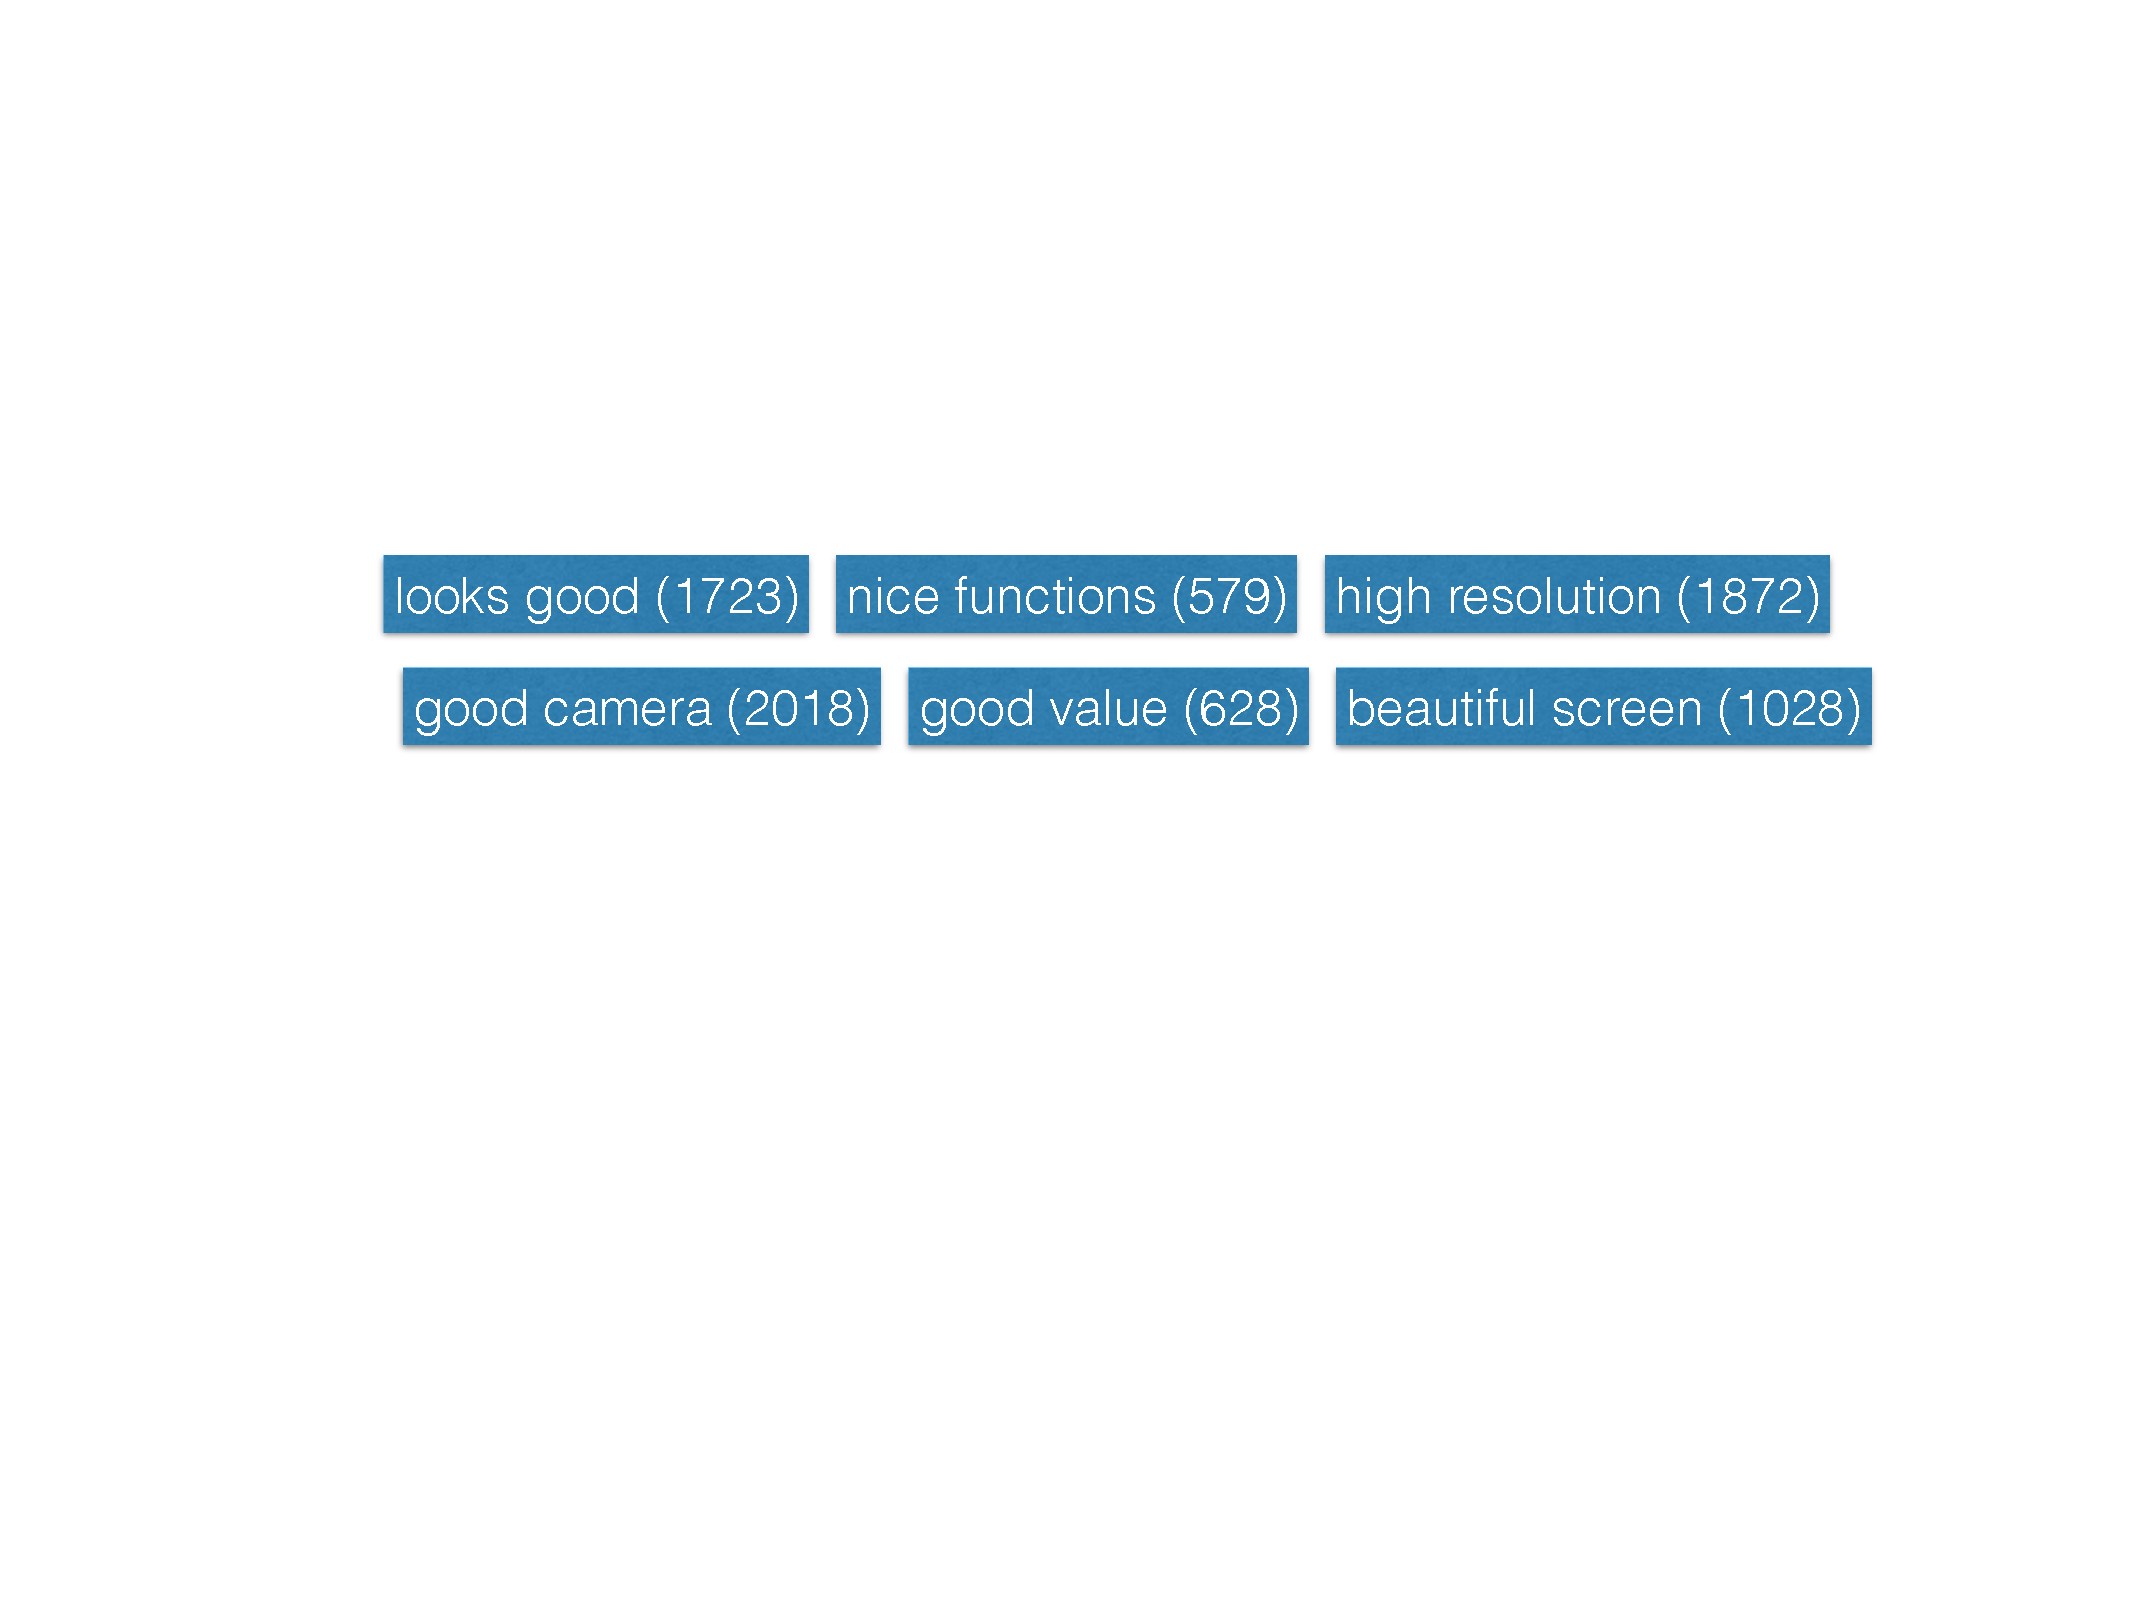
\includegraphics[width=0.7\columnwidth]{figures/experiments/opinion_phrases}
\caption{Opinion phrases given by the website.}
\label{fig:experiments:opinion_phrases}
\end{figure}

Here we explain how to use our frameworkd to construct a more informative, aspect-based summarization. We use the aspect clusters extracted by our model and identify the aspects in the sentences by checking if the top aspect words in each cluster appeared, if so, the sentence has a score equal to the highest aspect score it contains; the sentiment value of the sentence is predicted with an LSTM and feed-woward network model trained on Stanford Sentiment Treebank \cite{socher2013recursive}; the sentiment value for each aspect from the whole set is the average of the predicted sentiment values, averaged by the aspect scores of each sentence. 

\begin{figure}[t!]
\centering
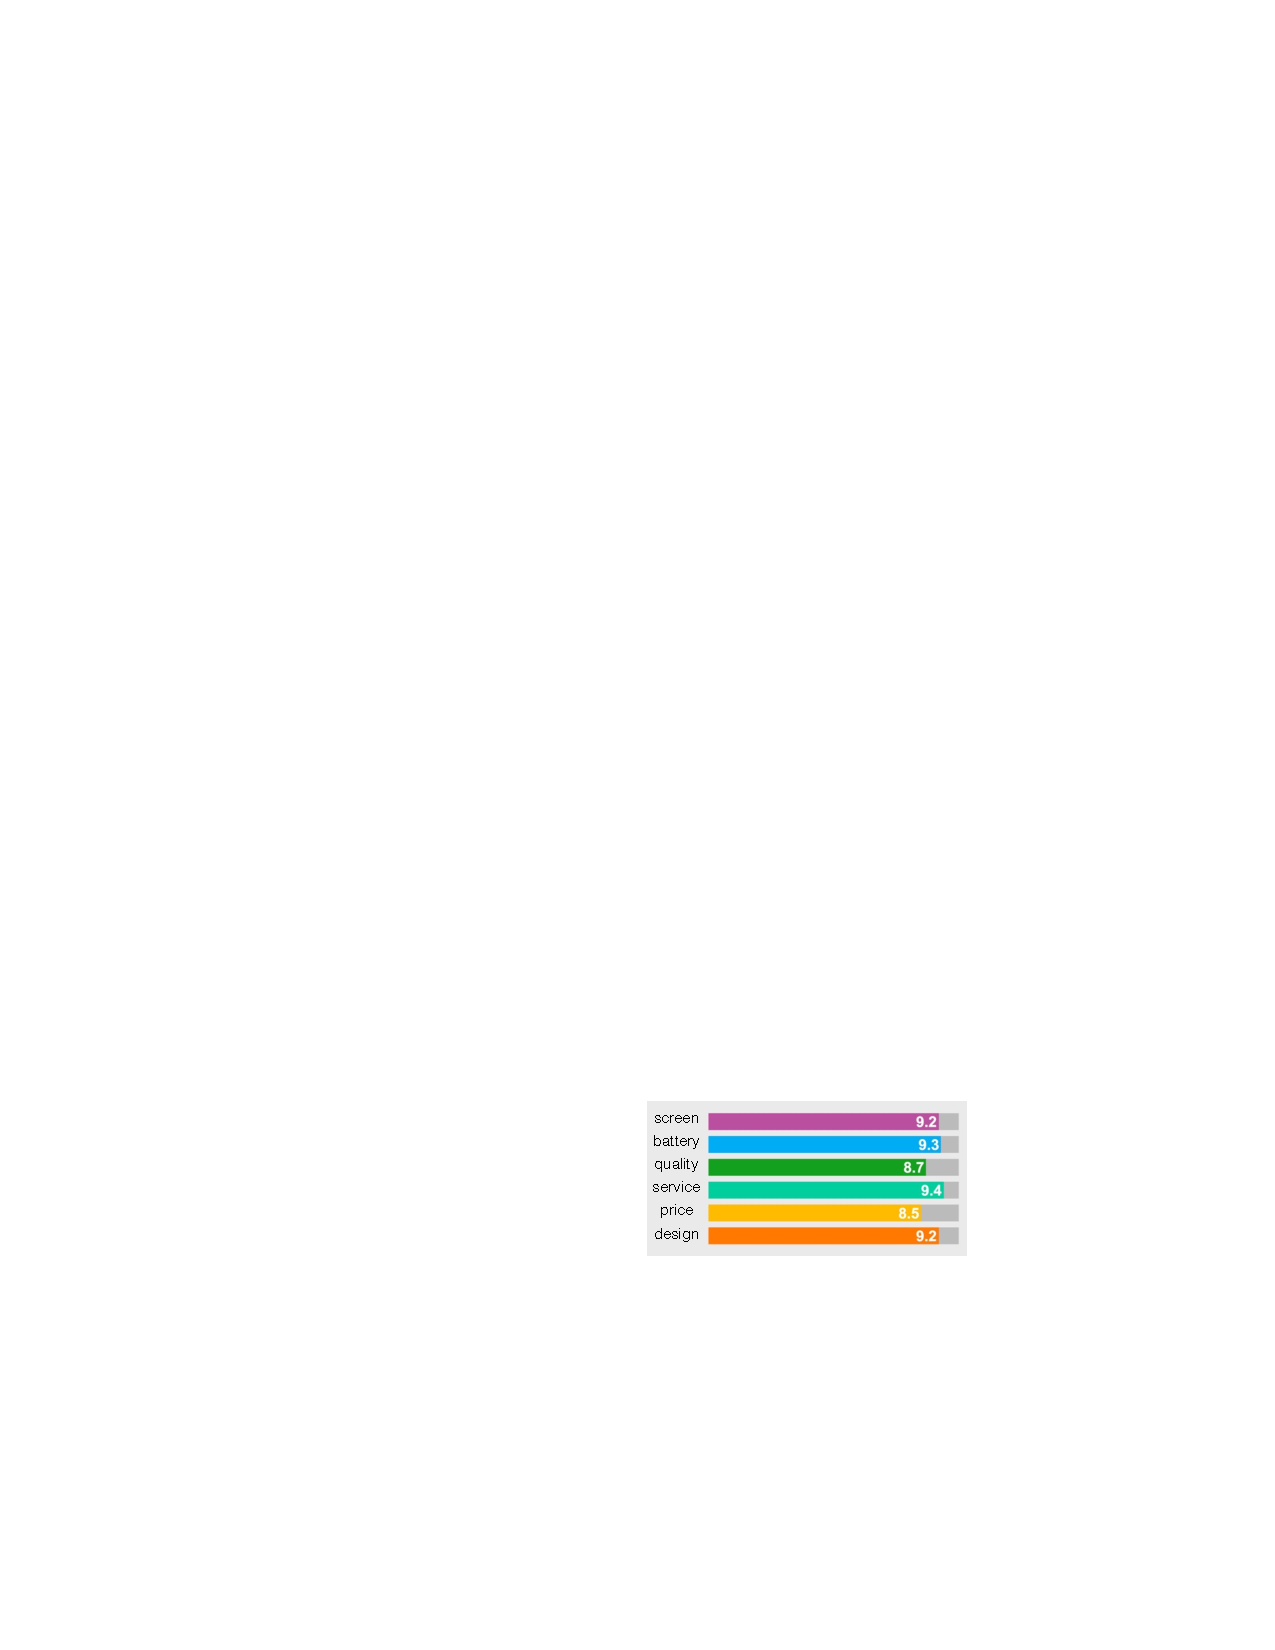
\includegraphics[width=0.5\columnwidth]{figures/experiments/scores}
\caption{Review summarization for iPhone 6.}
\label{fig:experiments:scores}
\end{figure}

The summarization produced by the said procedure on the same iPhone 6 review dataset is shown in Figure~\ref{fig:experiments:scores}. We take the top 6 aspect cluster as ranked by our ranking algorith; other than this, no manual process is involved. Our summarization is much more structured and informative, and different products in the same category can be easily compared in this form, because of the uniform format and quantitative scores, as shown in  Figure~\ref{fig:experiments:comparison}.

\begin{figure}[h!]
\centering
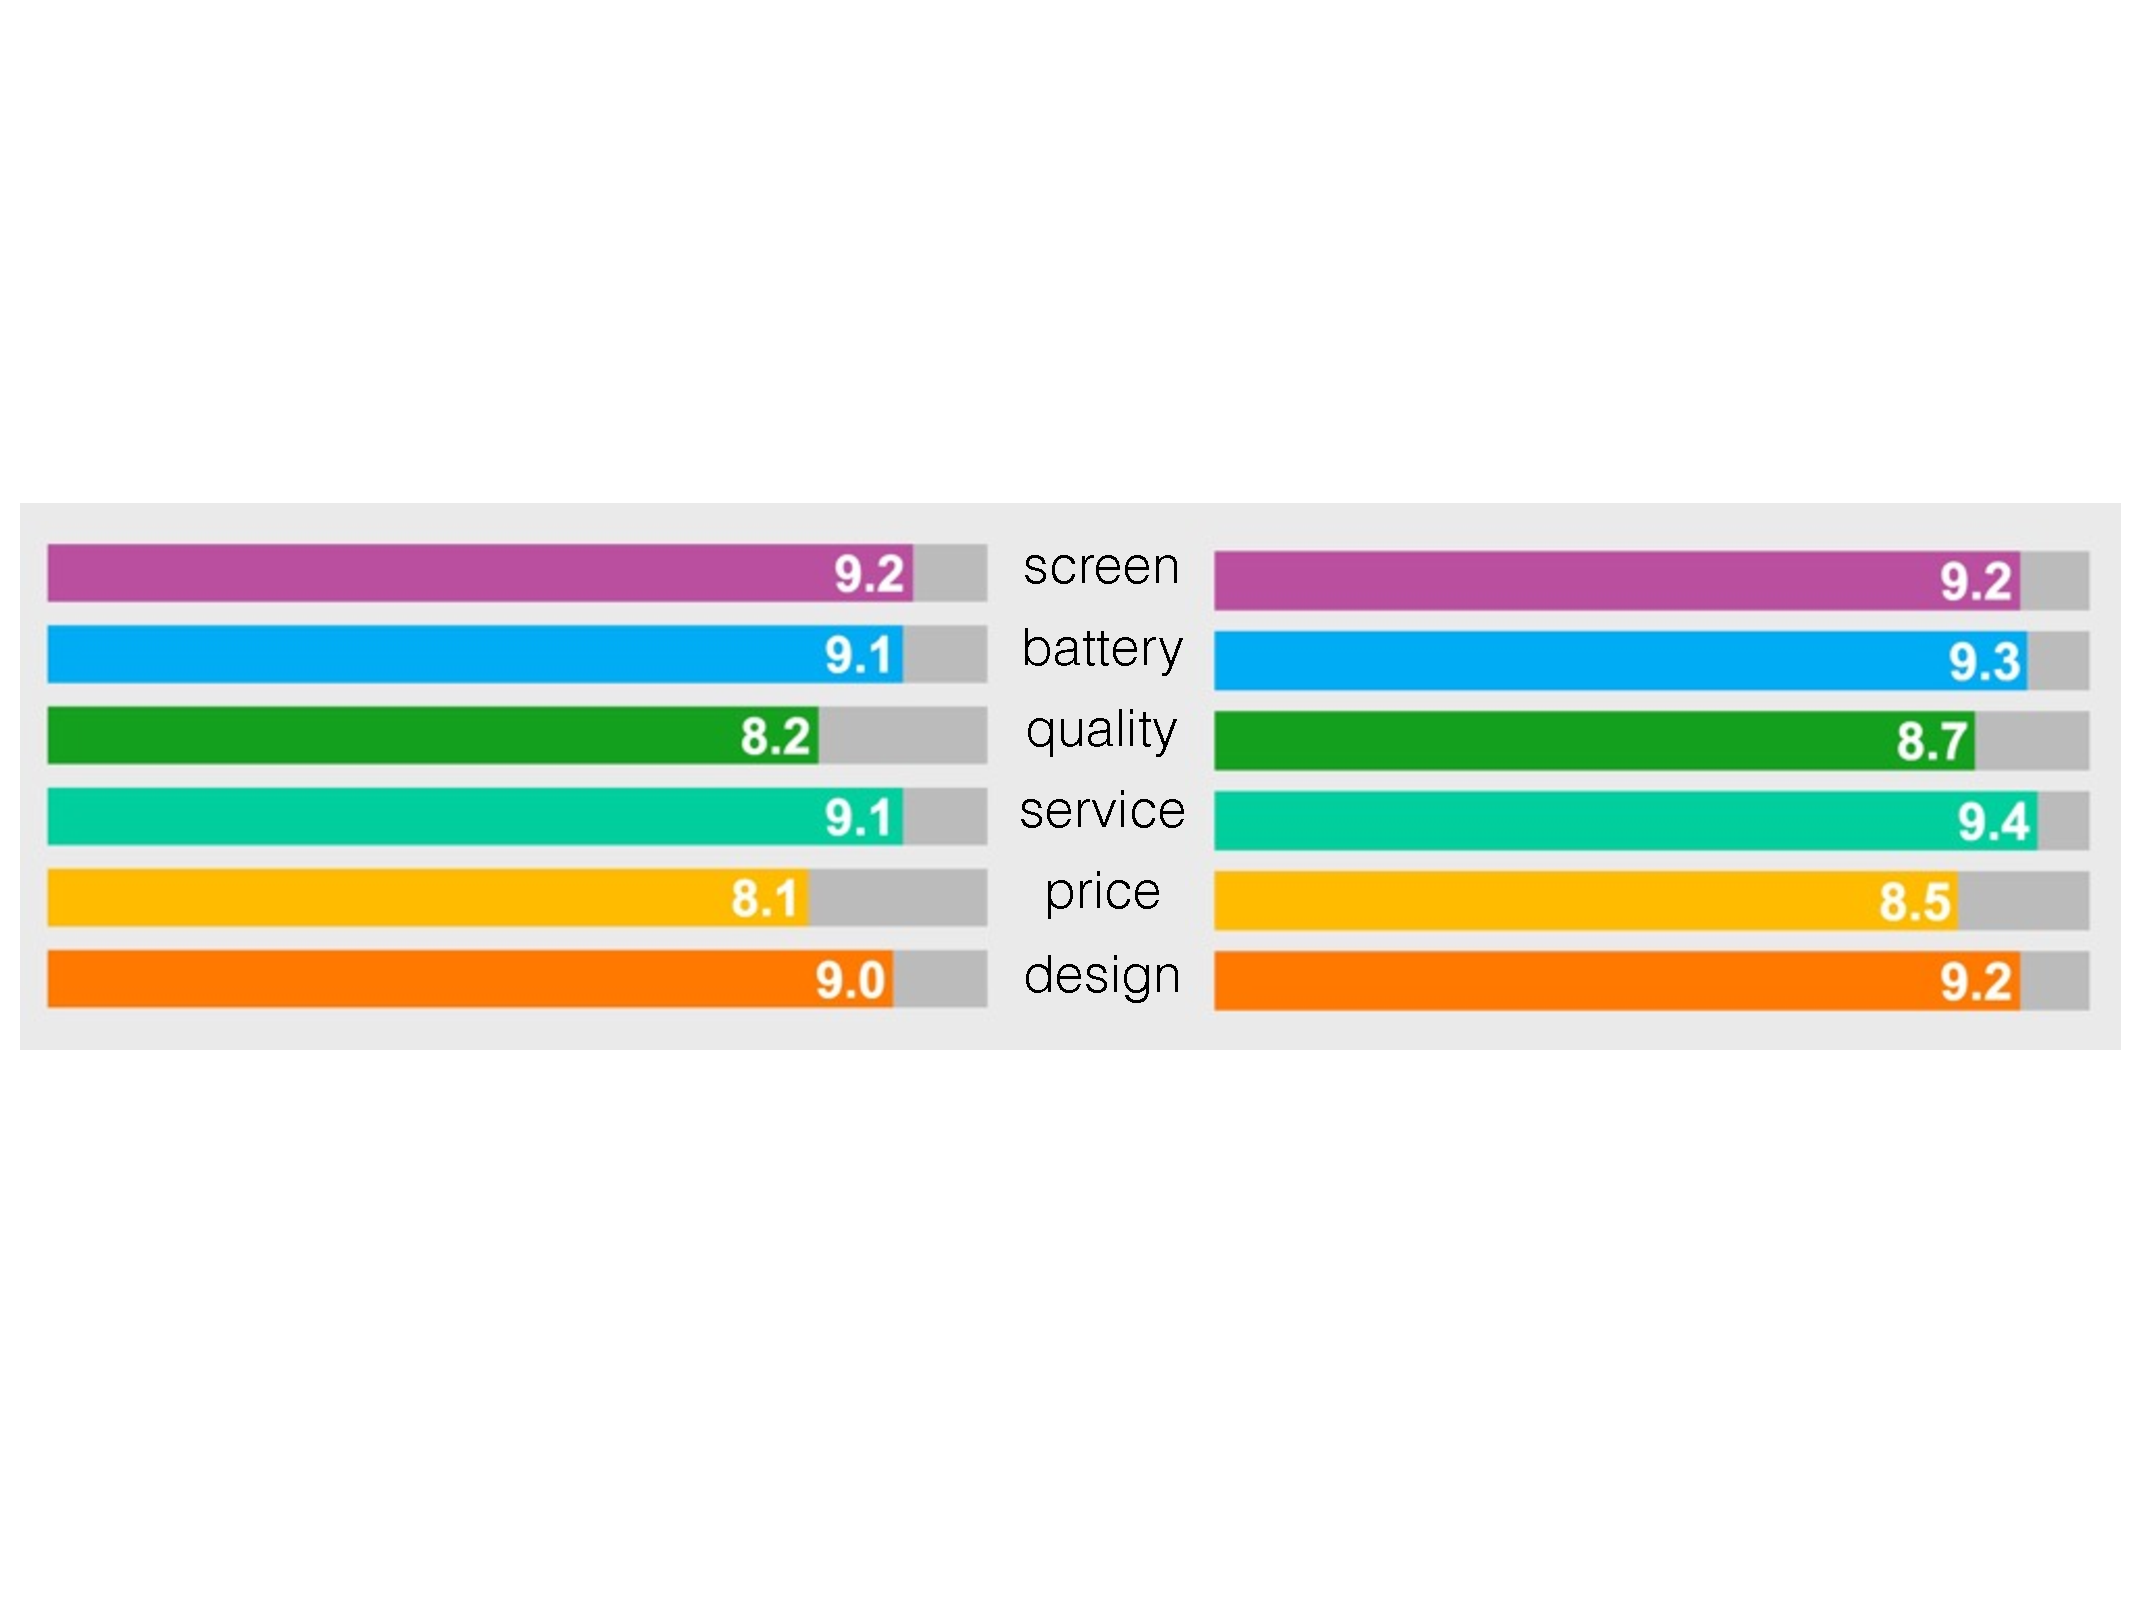
\includegraphics[width=1.0\columnwidth]{figures/experiments/comparison}
\caption{Comparing Galaxy S7 (left) with iPhone 6 (right).}
\label{fig:experiments:comparison}
\end{figure}

Another advantage of our method is that the chosen aspects reflect what the consumers care about each product. The fundamental reason behind this is that our model can truly leverage the huge amount of data compared to traditional methods. In Figure~\ref{fig:experiments:opinion_phrases}, we can see phrases ``beautiful screen" and ``good camera", but we also see ``high resolutin", which is confusing because we cannot know if it means the screen or the camera, and either way it is a duplication. In our method, the topics of the sentence is implicitly embedded in the sentence vector in the first clustering process, so we can leverage not only the opinion phrases but other surrounding words to decide whether ``high resolution" is talking about the screen or the camera, for example if the review sentence is ``it has high resolution and the texts look so crisp", we would know it's about the screen. This allows our summarization to leverage a lot more data than these traditional methods.
